\section{Cuestionario Previo}

\noindent \justifying

\subsection{¿Qué es la transformada de Laplace?}

Primero entendamos el concepto de transformación matemáticamente hablando.
"En cálculo elemental aprendió que la derivación y la integración son transformadas; esto significa, a grandes rasgos, que estas operaciones transforman una función en otra. Por ejemplo, la función $f(x)=x^{2}$ se transforma, a su vez, en una función lineal y en una familia de funciones polinomiales cúbicas con las operaciones de derivación e integración":


\begin{equation}
		\frac{d}{d x} x^{2}=2 x \hspace{1cm}
		\text { y } \quad \int x^{2} d x=\frac{1}{3} x^{3}+c
\end{equation}

Las dos anteriores operaciones son   tomadas textualmente del texto  porque es un excelente ejemplo para ponerte en contexto de las transformadas, además de explicar dos propiedades que heredan la la transformada de Laplace, que estan asociadas a que sea una transformada lineal.

\paragraph*{Propiedades de linealidad}

Propiedad  tal que la transformada de una combinación lineal de funciones es una combinación lineal de las transformadas. Para $\alpha$ y $\beta$ constantes

\begin{equation}
	\frac{d}{d x}[\alpha f(x)+\beta g(x)]=\alpha f^{\prime}(x)+\beta g^{\prime}(x)
	\label{propiedad_1}
\end{equation}

\begin{equation}
	\int[\alpha f(x)+\beta g(x)] d x=\alpha \int f(x) d x+\beta \int g(x) d x
	\label{propiedad_2}
\end{equation}

La transformada de Laplace tiene la propiedad [\ref{propiedad_1}] [\ref{propiedad_2}] , entre otras propiedades más interesantes, pero estas son las principales.


\paragraph*{Definición}
La transformada de Laplace es una formula para transformar una ecuación
diferencial que contiene las diferenciales de una función indefinida, a partir de una
ecuación t-espaciada hacia una ecuación s-espaciada que puede ser resuelta con mucha facilidad.	
\newline
La transformada de Laplace de una función \textit{f(t)} definida para todos los números positivos se define como:

\[
F(s) = \int_{0}^{\infty} \! e^{-st} f(t)  \,dt = \mathscr{L}\{f(t)\}
\]

\subsubsection{¿Para qué se utiliza?}
\noindent Esta transformada se usa para resolver:
 \begin{enumerate}
	\item Ecuaciones diferenciales de valor inicial (es necesario que tengan $n$ valores iniciales para una ecuación diferencial de orden $n$).
	\item Ecuaciones íntegro-diferenciales
\end{enumerate}

\noindent Se utiliza en:

\begin{enumerate}
	\item Servo sistemas.
	\item Análisis de circuitos electrónicos.
\end{enumerate}

\subsubsection{¿Cómo se construye la fórmula de Laplace?}


La definición de Laplace puede parecer difícil, ya que  no entendemos por que fue hecho de esta manera la ecuación, pero si nosotros entendemos el concepto de la transformada de Fourier, podremos entonces entender esto que yo entiendo como un concepto extendido de ella, ¿por qué digo que es una extensión? Fácil , tomamos la de Fourier  agregamos un termino a la ecuación para que pueda resolver ecuaciones diferenciales que la de Fourier no puede, es decir extendemos su funcionalidad, pero aparte da pie al concepto de \textbf{núcleo} en la transformada, si cambiamos ese término podremos resolver otros problemas.

Ahora mostraré como se pasa de la ecuación de Fourier a la ecuación de Laplace.

\begin{itemize}
	\item Kernel o núcleo es  $ e^{-\alpha \cdot t} $
\end{itemize}


\begin{equation}
		F(\omega)= \int^{\infty}_{- \infty} f(t)
	\underset{\substack{\downarrow \\ e{- \alpha t}}}{\cdot}
	e^{- j \omega t} dt
\end{equation}

\begin{equation}
	F(\omega)= \int^{\infty}_{- \infty} f(t)
	\underbrace{e^{- \alpha t} \cdot e^{- j \omega t}}_{e^{- (\alpha + j \omega)t}} dt 
	\label{furier_cambio}
\end{equation}

Realizamos un cambio de  variable  en la (\ref{furier_cambio}) , logrando que el cambio quede (\ref{furier_cambio2}).

\begin{equation}
	s= at + j \omega
	\label{furier_cambio2}
\end{equation}

\begin{equation}
	\int_{0}^{\infty} K(s, t) f(t) d t=\lim _{b \rightarrow \infty} \int_{0}^{b} K(s, t) f(t) d t
\end{equation}


\begin{equation}
	\mathscr{L}\{f(t)\}=\int_{0}^{\infty} e^{-s t} f(t) d t
\end{equation}

Una mejor explicación en el siguiente  \href{https://www.youtube.com/watch?v=i1wRqo\_2zgw}{(vídeo)}.

\subsubsection{Condiciones suficientes para la existencia}

¿Por qué digo que son condiciones suficientes , más no necesarias?. Existen ecuaciones que convergen a un valor y por ello es posible resolverlas por medio de Laplace aunque en el sentido estricto de las 2 siguientes condiciones , no es necesario que se cumplan.

\textbf{Condiciones :}
\begin{enumerate}
	\item Si $ f  $ es una función continua por tramos en $ [0, \infty) $.
	\subitem Veamos esta condición es algo peculiar , digamos  que nosotros en una función podemos tener puntos no esta definido como se aprecia en la gráfica \ref{fig:ilustracion1}. Nosotros podemos mover b , a la altura de a, y con ello hacer que la curva sea continua, a estos pequeños puntos se le llaman discontinuidades re movibles.
	\item  de orden exponencial c.
	\subitem Esta en resumen de cuentas es que el incremento de la función sea menor a una exponencial C multiplicada por otros factores, es como lo que hacíamos en cálculo integral, cuando comparábamos 2 funciones, si una convergía y la otra crecía menos que la que converge, entonces la otra converge.
\end{enumerate}

Si ambas condiciones se cumplen, entonces podemos afirmar que la transformada para la función existe.

\begin{figure}[h]
	\centering
	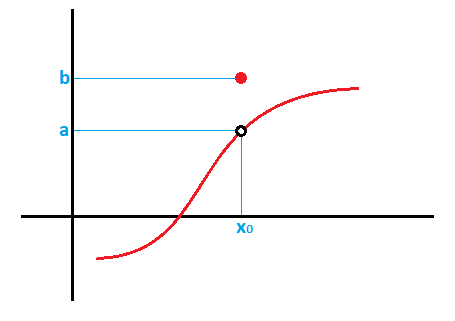
\includegraphics[width=0.7\linewidth]{img/ilustracion_1}
	\caption{Gráfica con discontinuidad re movible}
	\label{fig:ilustracion1}
\end{figure}


\subsection{¿Qué es la función de transferencia y cómo puede ser determinada?}	
La función de transferencia es una representación conveniente de un sistema dinámico de tiempo lineal invariable. Para sistemas de dimensiones finitas la función de transferencia es simplemente una función racional que representa a relación que hay entre la transformada de Laplace de la salida (respuesta de estado cero) y la entrada del sistema. Esta función se puede obtener tanto por inspección como por una manipulación algebraica de las ecuaciones diferenciales que describen el sistema. Su importancia es que permite analizar funciones de un orden muy alto, e incluso puede analizar funciones de dimensiones infinitas si son sistemas gobernados por ecuaciones diferenciales parciales. Cabe recalcar que para que dicha función tenga un significado, el sistema analizado debe de ser lineal, invariante en el tiempo y con condiciones iniciales nulas. La función de transferencia está representada por la siguiente ecuación:

\begin{equation} 
	H(s)=\frac{Y_{sz}(s)}{X(s)}
\end{equation}

\noindent Donde:
\begin{itemize}
	\item $Y_sz(s)$ es la transformada de Laplace de la respuesta de estado cero $y_{sz}(t)$	
	\item $H(s)$ es la transformada de Laplace de la respuesta al impulso $h(t)$
	\item $X(s)$ es la transformada de Laplace de la entrada $x(t)$
\end{itemize}

\noindent\textbf{Obtención de la función de transferencia}
\newline

Sea la ecuación diferencial lineal de coeficientes constantes de orden N que describe al sistema la transformada de Laplace correspondiente resulta

\begin{equation}
	\Laplace\{\sum_{n=0}^{N} a_n \frac{d^ny(t)}{dt^n} \}  = \Laplace\{\sum_{n=0}^M a_n \frac{d^nx(t)}{dt^n} \}
\end{equation}

\noindent Aplicando la propiedad de derivación a la ecuación anterior se obtiene

\begin{equation}
	\sum_{n=0}^M a_ns^nY(s)\ - \sum_{n=1}^N a_n\{ \sum_{m=1}^n y^{m-1}(0^-)s^{s-m} \}\ = \sum_{n=0}^Mb_ns^xX(s) - \sum_{n=1}^M b_n\{ \sum_{m=1}^M x^{m-1}(0^-)s^{s-m} \}\
\end{equation}

\noindent Donde $y^{m-1}(0^-)$ y 	$x^{m-1}(0^-)$ son las (m-q)-ésimas derivadas de y(t) y x(t) evaluadas en $t=0^-$, respectivamente. Si despejamos a Y(s) obtenemos:

\begin{equation}
	Y(s)=\frac{\sum_{n=0}^Mb_ns^xX(s) - \sum_{n=1}^M b_n\{ \sum_{m=1}^M x^{m-1}(0^-)s^{s-m} \}}{\sum_{n=0}^Na_ns^n} + \frac{\sum_{n=1}^N a_n\{ \sum_{m=1}^n y^{m-1}(0^-)s^{s-m} \}}{\sum_{n=0}^Na_ns^n}
\end{equation}

\noindent Como se ha mencionado, si el sistema en estudio está en reposo, las condiciones iniciales son nulas y por consiguiente la respuesta a la ecuación anterior es nula, de igual manera el término de la respuesta detestado cero relacionado con sus respectivas condiciones iniciales, reduciéndose a 

\begin{equation}
	Y_{zs}(s)=\frac{\sum_{n=0}^M b_ns^nX(s)\ }{\sum_{n=0}^Na_ns^n\ }
\end{equation}

\noindent La \textit{función de transferencia} se define como la razón de la transformada de la salida a la transformada de la entrada cuando todas las condiciones iniciales son cero. Así

\begin{equation}
	H(s)=\frac{Y_{zs}(s)}{X(s)} = \frac{\sum_{n=0}^M b_ns^n}{\sum_{n=0}^M a_ns^n}
\end{equation}

\noindent Que igualmente se puede representar de la siguiente forma

\begin{equation}
	H(s)=\frac{Y_{zs}(s)}{X(s)} = \frac{K(s+q_0)(s+q_1)···(s+q_M)}{s+p_0)(s+p_1)···(s+p_M)} = \frac{Q(s)}{P(s)}
\end{equation}

\noindent La expresión anterior es la representación general de un sistema que en el domino del tiempo ecuación diferencial lineal de coeficientes constantes de orden N.
\subsection{¿Qué es un polo y qué es un cero? y ¿cómo pueden ser determinados?.}


Dada a una función de transformación continua, en el dominio de Laplace, \textit{H(s)}, o en el dominio discreto de Z, \textit{H(z)}, un cero es cualquier valor de s o z para los cuales la función de transferencia es cero, un polo es cualquier valor de s o z para la cual la función de trasferencia es infinita.\newline
En otras palabras el cero es el valor(es) para \textit{z} en donde el numerador de la función de trasferencia es iguala cero. Y el polo es el valor(es) para \textit{z} donde el denominador de la función de transferencia es igual a cero.

\[
H(s) = \frac{Numerador = 0 \textit{ CEROS} }{Denominador = 0 \textit{ POLOS}}
\]
\newline
Para poder determinar los ceros de en una función de transferencia, lo único que debemos de hacer es factorizar, o lo que es lo mismo, encontrar las raíces del polinomio del \textit{numerador} igualado a 0.\newline
De la misma manera vamos a encontrar los polos de una función de transferencia, solo que esta vez vamos a factorizar el polinomio del \textit{denominador} igualado a 0. Las raíces obtenidas van a ser los ceros o polos según sea el caso.\\


